\documentclass[a4paper]{article}
\usepackage{inputenc}
\usepackage[british,UKenglish]{babel}
\usepackage{amsmath}
\usepackage{titlesec}
\usepackage{color}
\usepackage{graphicx}
\usepackage{fancyref}
\usepackage{hyperref}
\usepackage{float}
\usepackage{scrextend}
\usepackage{setspace}
\usepackage{xargs}
\usepackage{multicol}
\usepackage{nameref}
\usepackage{sectsty}
\usepackage{multicol}
\usepackage{multirow}
\usepackage[procnames]{listings}
\usepackage{appendix}
\usepackage{listings}
\usepackage{fancyhdr}
\usepackage[UTF8]{ctex}
\usepackage{geometry}
\usepackage{multirow}
\usepackage{tikz}
\usepackage{xeCJK}

\setmainfont{Times New Roman}
\setCJKmainfont[BoldFont=Source Han Serif SC SemiBold]{Source Han Serif SC}
% \setCJKsansfont{Heiti SC}
% \setCJKmonofont{Courier}

\newcommand\tab[1][1cm]{\hspace*{#1}}
\hypersetup{colorlinks=true, linkcolor=black}
\interfootnotelinepenalty=10000

\newcommand{\cleancode}[1]{\begin{addmargin}[3em]{3em}\texttt{\textcolor{cleanOrange}{#1}}\end{addmargin}}
\newcommand{\cleanstyle}[1]{\text{\textcolor{cleanOrange}{\texttt{#1}}}}

\usepackage[colorinlistoftodos,prependcaption,textsize=footnotesize]{todonotes}
\newcommandx{\commred}[2][1=]{\textcolor{Red}
{\todo[linecolor=red,backgroundcolor=red!25,bordercolor=red,#1]{#2}}}
\newcommandx{\commblue}[2][1=]{\textcolor{Blue}
{\todo[linecolor=blue,backgroundcolor=blue!25,bordercolor=blue,#1]{#2}}}
\newcommandx{\commgreen}[2][1=]{\textcolor{OliveGreen}{\todo[linecolor=OliveGreen,backgroundcolor=OliveGreen!25,bordercolor=OliveGreen,#1]{#2}}}
\newcommandx{\commpurp}[2][1=]{\textcolor{Plum}{\todo[linecolor=Plum,backgroundcolor=Plum!25,bordercolor=Plum,#1]{#2}}}

\def\code#1{{\tt #1}}

\def\note#1{\noindent{\bf [Note: #1]}}

\makeatletter
%% The "\@seccntformat" command is an auxiliary command
%% (see pp. 26f. of 'The LaTeX Companion,' 2nd. ed.)
\def\@seccntformat#1{\@ifundefined{#1@cntformat}%
   {\csname the#1\endcsname\quad}  % default
   {\csname #1@cntformat\endcsname}% enable individual control
}
\let\oldappendix\appendix %% save current definition of \appendix
\renewcommand\appendix{%
    \oldappendix
    \newcommand{\section@cntformat}{\appendixname~\thesection\quad}
}
\makeatother

\geometry{a4paper, left=2.5cm, right=2.5cm, top=2.5cm, bottom=2.5cm}

\lstset{
  frame=lines,
  rulesepcolor=\color{red!20!green!20!blue!20},
  numbers=left,
  numberstyle=\small,
  breaklines=true,
  escapebegin=\begin{CJK*},
  escapeend=\end{CJK*},
  basicstyle=\ttfamily,
  keywordstyle=\color{green!40!black},
  identifierstyle=\color{blue!60!black},
  stringstyle=\color{red},
  commentstyle=\color{purple!40!black},
}

\newcommand\filecode[1]{\lstinputlisting[xleftmargin=5mm, xrightmargin=5mm]{#1}}

% page head
\fancypagestyle{preContent}{
  \fancyhf{}
  \renewcommand\headrulewidth{.5pt}
  \renewcommand\footrulewidth{0pt}
  \fancyhead[OC]{\textcolor{gray}{this is a example page head}}
  \fancyfoot[C]{\thepage}
}
\pagestyle{preContent}


% include images
\graphicspath{ {figures/} }

\begin{document}
\renewcommand{\contentsname}{目\ 录}
\renewcommand{\appendixname}{附录}
\renewcommand{\appendixpagename}{附录}
\renewcommand{\refname}{参考文献} 
\renewcommand{\figurename}{图}
\renewcommand{\tablename}{表}
\renewcommand{\today}{\number\year 年 \number\month 月 \number\day 日}

\begin{titlepage}
\begin{center}
  \vspace*{36pt}
  \fontsize{48pt}{0}{\textbf{标题}} \\
  \vspace*{24pt}
  \fontsize{42pt}{0}{\textbf{实验报告}} \\
  \vspace*{380pt}
\end{center}
\date{\today}
\author{wjl}
\end{titlepage}
\newpage

\tableofcontents

\newpage

\section{第一章}\label{sec1}

这里是第一章内容

行内公式 $a + b - c + d = e$

\[
y = \lim_{n \to \infty} \frac{1}{n}  
\]

\section{第二章}\label{sec2}

这里是第二章内容

\subsection{第一节}\label{sec2:sub1}

C++ 代码块

\begin{lstlisting}[language=c++]
#include <iostream>
int main() {
  std::cout << "Hello World!\n";
}
\end{lstlisting}

Java 代码块

\begin{lstlisting}[language=java]
public class Main {
  public static void main(String[] args) {
    System.out.println("Hello World!");
  }
}
\end{lstlisting}

\subsection{第二节}\label{sec2:sub2}

图片

\begin{figure}[ht]
  \centering
  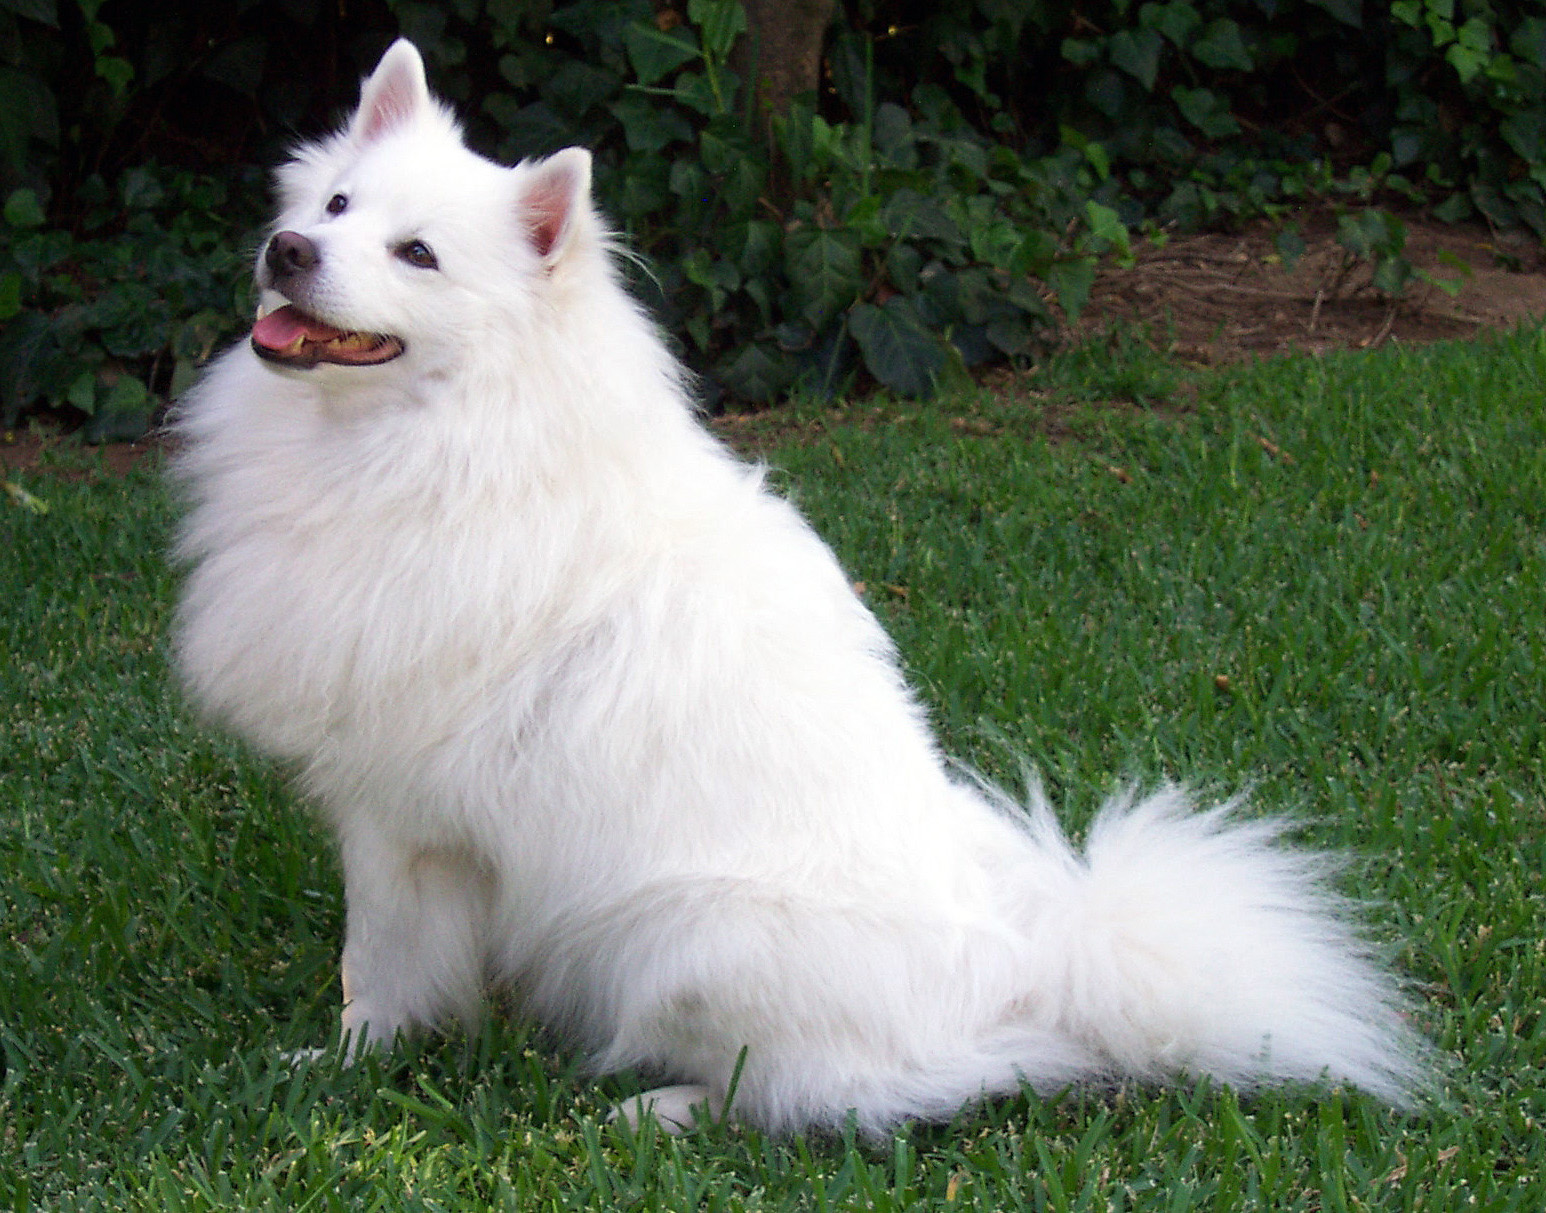
\includegraphics[height=5cm]{figures/dog.png}
  \caption{小狗}
  \label{fig:dog}
\end{figure}

\subsection{第三节}\label{sec2:sub3}

\section{第三章}\label{sec3}

\begin{thebibliography}{9}

\bibitem{01} 参考文献1
\bibitem{02} 参考文献2

\end{thebibliography}

\end{document}
